\documentclass{beamer}
\usetheme{metropolis}
\usepackage{amssymb}
\usepackage{appendixnumberbeamer}
\usepackage{tabu}
\usepackage{listings}
\usepackage{hyperref}
%\usepackage{pgfplotsthemetol}
\hypersetup{colorlinks=true}

\newcommand{\jumbotron}[1]{ \centering \LARGE{#1} }
\newcommand{\citebook}{\tiny{Source: \emph{Introduction to Reproducible Science in R} -- Brian Lee Yung Rowe}}

\definecolor{graydark}{rgb}{0.3,0.3,0.3}
\definecolor{graymedium}{rgb}{0.5,0.5,0.5}
\definecolor{graylight}{rgb}{0.7,0.7,0.7}

\lstloadlanguages{bash}
\lstdefinestyle{custombash}{
  language=bash,
  frame=bt,
  otherkeywords={$},
  numberstyle=\tiny\color{graymedium},
  basicstyle=\footnotesize\ttfamily,
  stringstyle=\color{graydark},
  commentstyle=\color{graymedium},
  keywordstyle=\textbf\ttfamily,
  showstringspaces=false,
  numbers=left,
  breaklines=true
}


\title{Process Automation as the Backbone of Reproducible Science} 
\date{\today} 
\author{Brian Lee Yung Rowe} 
\institute{Founder \& CEO, Pez.AI\\ CEO, FundKo} 

\begin{document} 
\maketitle 

\section{Introduction} 
\begin{frame}{About Me}

\begin{itemize}
\item Founder \& CEO of \href{https://pez.ai}{Pez.AI}, productivity chatbots that make communication and coordination more efficient
\item CEO of \href{https://fundko.com}{FundKo}, P2P lender in Philippines using behavioral economics to improve lending outcomes
\item Author of \emph{Introduction to Reproducible Science in R}, to be published by Chapman and Hall/CRC Press
\item 6 years adjunct: NLP, machine learning, predictive analytics, mathematics
\item 14 years quantitative finance/investment management
\end{itemize}
\end{frame} 


\begin{frame}{Outline}
\begin{itemize}
\item Why reproducible science?
\item Process automation: code as methodology
\item Process automation: computing environment
\item Pearls of wisdom

\end{itemize} 
\end{frame} 


\section{Why Reproducible Science}

\begin{frame}{What is truth?}
Does hydroxychloroquine increase mortality rate of COVID-19?


\includegraphics[width=6cm]{images/hydroxychloroquine}

\end{frame}


\begin{frame}{Which is correct?}
\begin{columns}
\begin{column}{.5\textwidth}
22 May (Lancet, NEJM):


\includegraphics[trim=0 7mm 0 9mm,clip, width=\linewidth]{images/yes}

(\href{https://www.theguardian.com/world/2020/jun/03/covid-19-surgisphere-who-world-health-organization-hydroxychloroquine}{Source})
\end{column}

\begin{column}{.5\textwidth}
\pause
2-3 June (\href{https://www.thelancet.com/journals/lanpub/article/PIIS0140-6736(20)31290-3/fulltext}{Lancet}, \href{https://www.nejm.org/doi/full/10.1056/NEJMe2020822?query=featured\%E2\%80\%94coronavirus}{NEJM}):

\includegraphics[width=\linewidth]{images/actually}

(\href{https://www.theguardian.com/world/2020/jun/03/how-were-medical-journals-and-who-caught-out-over-hydroxychloroquine}{Source})
\end{column}
\end{columns}

% https://people.com/health/who-suspends-hydroxychloroquine-trials-after-reports-of-high-death-rates-in-covid-19-patients/
%https://www.thelancet.com/journals/laninf/article/PIIS1473-3099(20)30313-3/fulltext
%https://www.reuters.com/article/us-health-coronavirus-indonesia-chloroqu-idUSKBN23227L
\end{frame}



\begin{frame}{Reproducing results is hard}
\centering

%Results are notoriously difficult to reproduce\onslide<2->{, leading to skepticism, mistrust, unnecessary suffering}

% https://www.cnn.com/2020/03/23/health/chloroquine-hydroxycholoroquine-drugs-explained/index.html
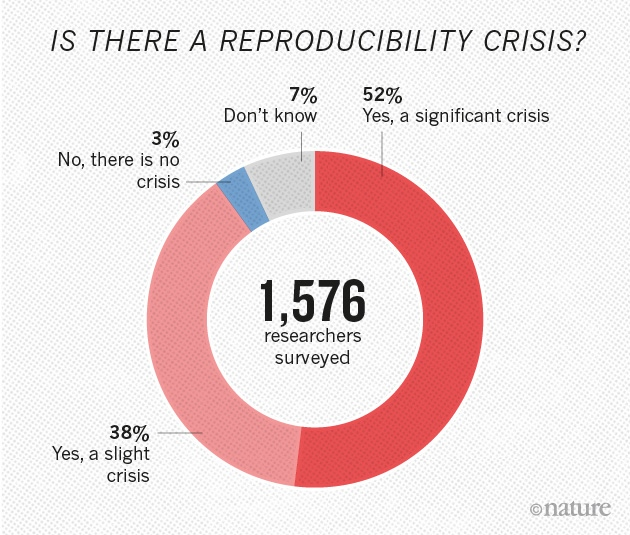
\includegraphics[width=.6\linewidth]{images/reproducibility_nature}\\
\footnotesize{Source: \href{https://www.nature.com/news/1-500-scientists-lift-the-lid-on-reproducibility-1.19970}{Nature}}

\end{frame}



\begin{frame}{Truth as a gradient}
Truth only exists when claims can be confirmed

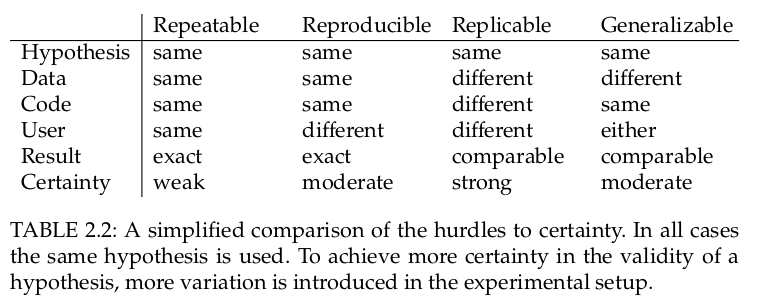
\includegraphics[width=\linewidth]{images/reproducibility_table}\\
\citebook ~ (based on NSF definitions)
\end{frame}


\begin{frame}{Example: Computer Vision/Image Classification}

%Repeatability - same ingredients, same recipe, same cook
%Reproducibility - same ingredients, same recipe, different cook
%Replicability - similar ingredients, similar recipe, different cook
%Generalizability - different ingredients, same recipe -> different result (pajun vs pancake)


%ingredients - data\\
%recipe - model

%https://www.gordonramsayrestaurants.com/recipes/buttermilk-pancakes/
\small
\centering
\begin{tabu} to \linewidth{c|c}
Repeatable & Reproducible\\
%(me: my code, data) & (you: my code, data)\\
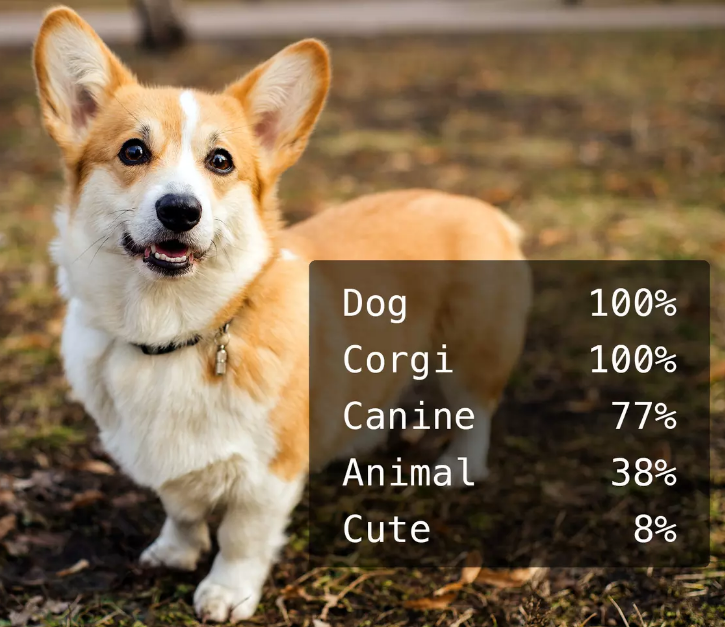
\includegraphics[width=.3\linewidth]{images/dog} &
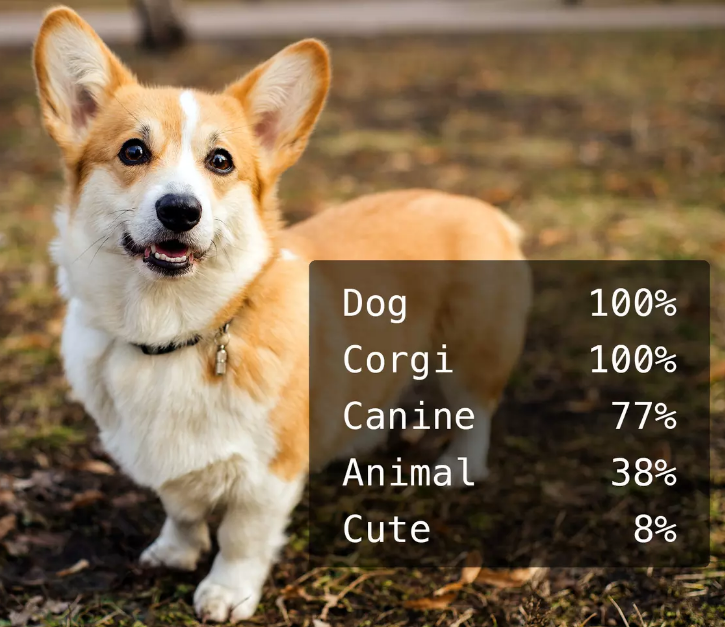
\includegraphics[width=.3\linewidth]{images/dog} \\
\hline
Replicable & Generalizable (FAIL)\\
%(you: your code, my data) & (my code, your data) \\
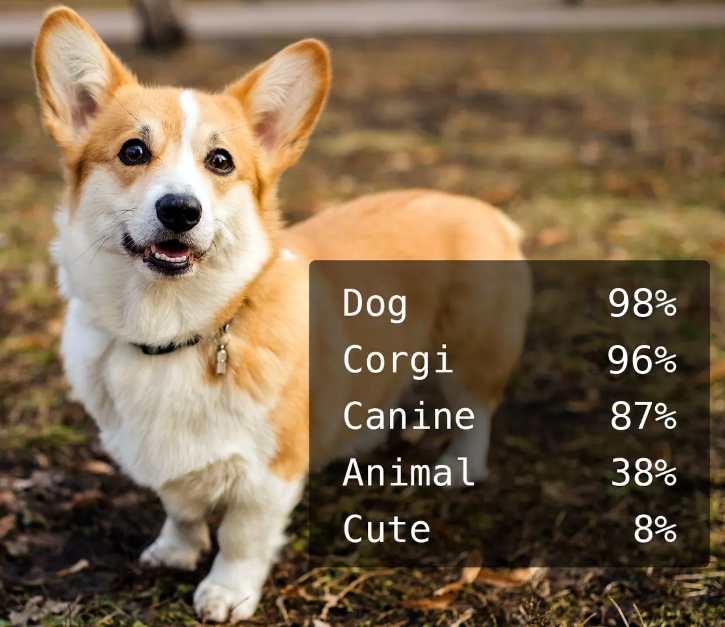
\includegraphics[width=.3\linewidth]{images/dog_replicable} &
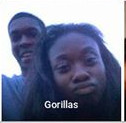
\includegraphics[trim={0 0 3mm 0},clip, width=.3\linewidth]{images/gorilla_fail}
\end{tabu}

%https://cdn.quotesgram.com/img/15/65/663056755-Qvc_swedish_chef_kitchen.jpg

%https://www.gordonramsayrestaurants.com/assets/Uploads/_resampled/CroppedFocusedImage108081050-50-buttermilk-pancake-recipe.jpg


%http://dinnerandconversation.com/2010/05/strawberry-souffle-disaster-recipe.html
\end{frame}


\begin{frame}{Factors Driving Reproducibility}

\centering
%of methodology and environment
Research is more reproducible when methodology and environment 
are \alert{transparent} and \alert{accessible}

\begin{align}
%reproducibility \sim transparency + accessibility
reproducibility \sim methodology + environment
\end{align}

\end{frame}



\begin{frame}{Opaque Methodology}
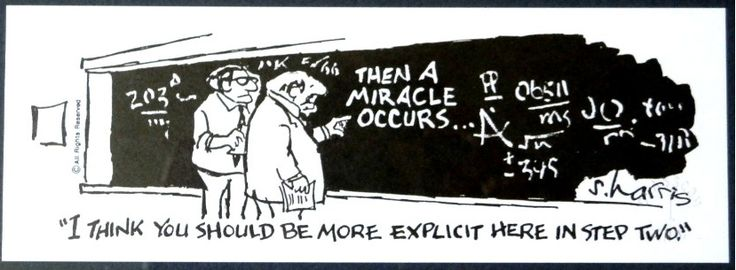
\includegraphics[width=\linewidth]{images/thenamiracleoccurs}
%https://noncon.files.wordpress.com/2015/10/thenamiracleoccurs.jpg
%Sidney Harris

\begin{itemize}
\item vague/no documentation
\item vague/undocumented data lineage and provenance
\item undocumented assumptions
\item manual steps
\item spaghetti code
\end{itemize}
\end{frame}



%\begin{frame}{Methodology}
%\begin{itemize}
%\item Experiment design - data acquisition, construction 
%\item Data analysis - filtering/censoring, correction, imputation, transformation, feature construction, model, training, validation
%\item Software development - design, building, testing, versioning, deploying
%\end{itemize}
%
%\end{frame}


\begin{frame}{Inaccessible Environment}
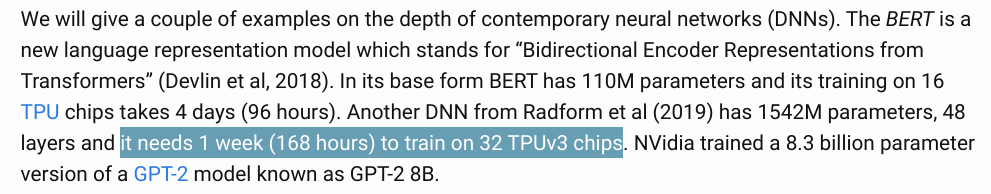
\includegraphics[width=\linewidth]{images/dl_training}

\tiny
(Source: \href{https://ekamperi.github.io/machine\%20learning/2019/08/14/energy-considerations-dnn.html}{Energy considerations for training deep neural networks})

\normalsize
\href{https://cloud.google.com/tpu/pricing}{Cost}: \$32/hour * 168 hours = \$5376

\begin{itemize}
\item massive system requirements
\item esoteric system requirements
\item esoteric dependencies
\item non-free data/tools
\end{itemize}

\end{frame}

%\begin{frame}{Environment}
%\begin{itemize}
%\item Where we conduct experiments: physical, computing
%\item Tools we use
%\item Initial conditions
%\end{itemize}

%\end{frame}



\section{Process Automation: Methodology}

\begin{frame}{Reproducibility as optimization problem}
Objective: minimize time to reproduce results

\begin{align}
\mbox{min} ~ reproduce(env, method)
\end{align}
s.t.\\ \mbox{env, method are transparent and accessible}

\end{frame}



\begin{frame}{The Data Science Paradox}
The worse you are at programming, the more time you spend doing it.
\begin{align}
t_{coding} \sim skill_{coding}
\end{align}

\pause
Corollary
\begin{align}
bugs \sim skill_{coding} + testing
\end{align}

\pause
Conclusion: Rigorous software development practice is required for reproducibility

\end{frame}



\begin{frame}{Code \emph{Is} Your Methodology}

\begin{columns}
\begin{column}{.5\linewidth}
Transparent and accessible code is easier to understand,
faster to confirm, identify, troubleshoot bugs
and \alert{avoids unnecessary retractions}.
\end{column}


\begin{column}{.5\linewidth}
% https://science.sciencemag.org/content/314/5807/1875.2
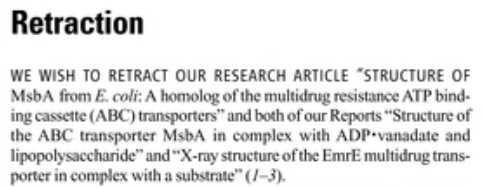
\includegraphics[width=\linewidth]{images/retraction_2}

~\\

% https://journals.sagepub.com/doi/10.1177/0022146515595817
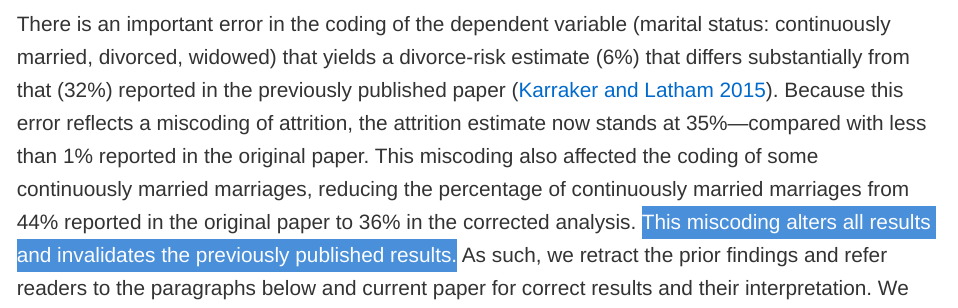
\includegraphics[width=\linewidth]{images/retraction_1}

~\\

% https://bmcbioinformatics.biomedcentral.com/articles/10.1186/1471-2105-5-80

\includegraphics[width=\linewidth]{images/retraction_3}
\end{column}
\end{columns}


%A little detective work traced the problem to default date format conversions and floating-point format conversions in the very useful Excel program package. The date conversions affect at least 30 gene names; the floating-point conversions affect at least 2,000 if Riken identifiers are included. These conversions are irreversible; the original gene names cannot be recovered.
%\pause
%\centering
%\begin{tikzpicture}
%\node (n) at (0,1) {$16$};
%\node (d) at (0,0) {$64$};
%\draw (-.4, .5) -- (.4, .5);
%
%\pause
%\draw (0, .8) -- (.2, 1.2);
%\draw (-.2, -.2) -- (0, .2);
%
%\pause
%\node (e) at (.9,.5) {$= \frac{1}{4}$};
%\end{tikzpicture}

\end{frame}


%\begin{frame}{Process Automation }
%\begin{tikzpicture}
%\node[inner sep=0pt] (game) at (0,0) {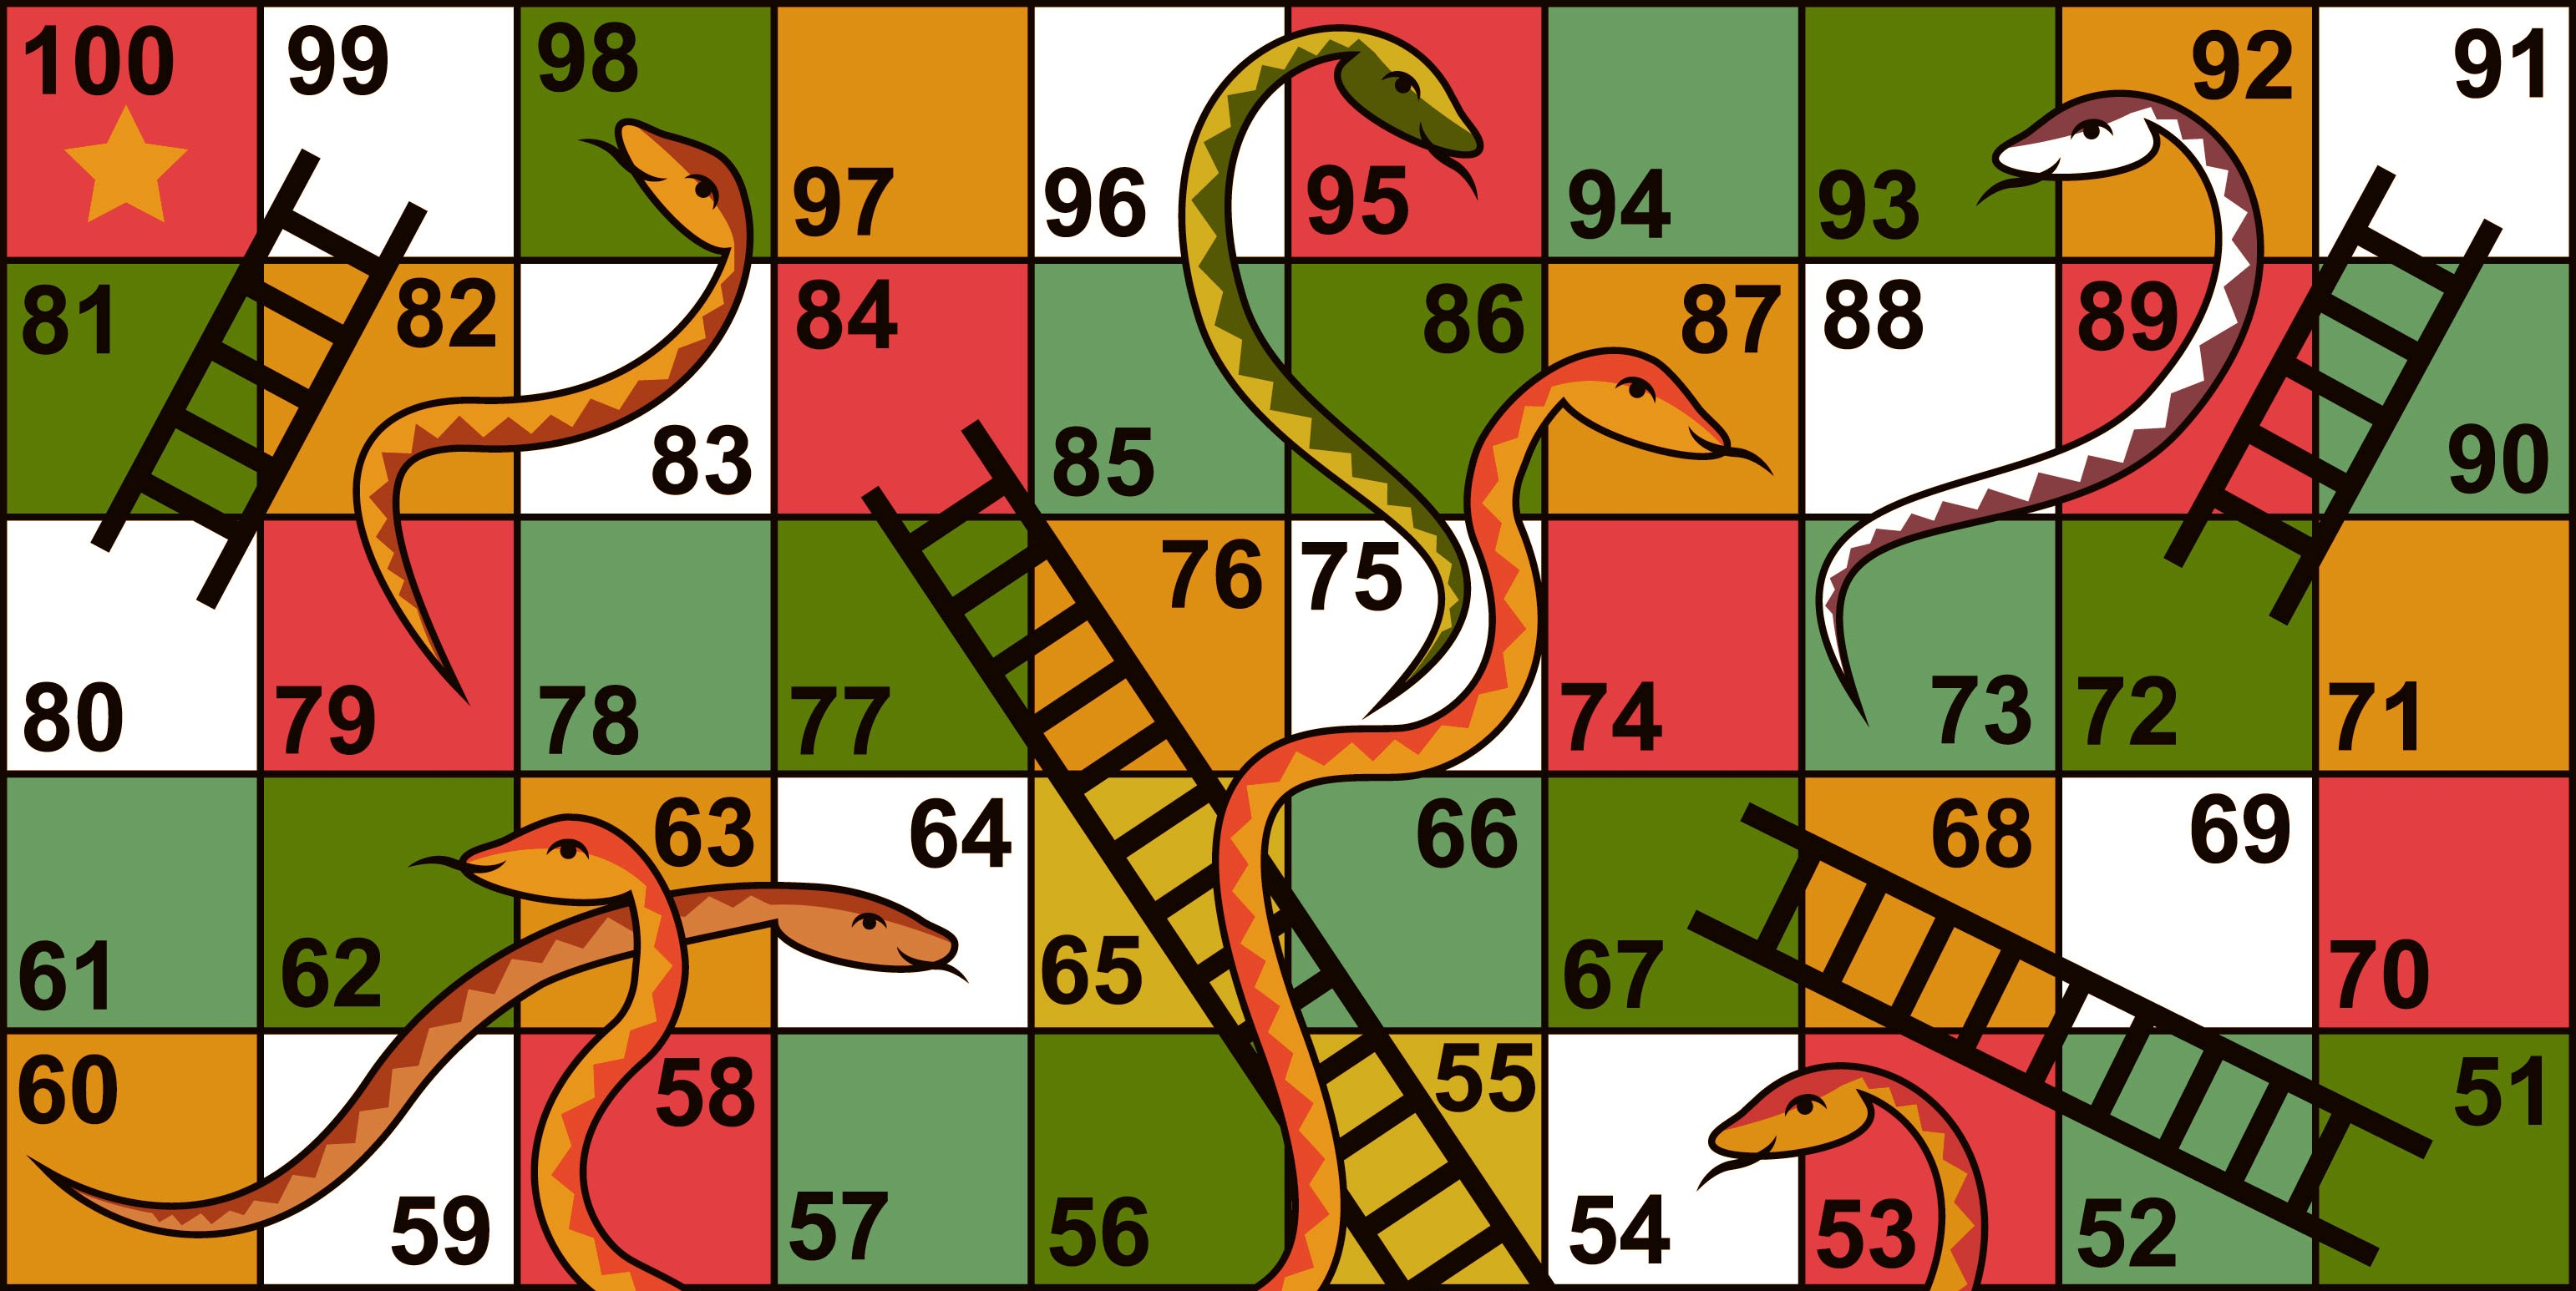
\includegraphics[width=\linewidth]{images/snakes_ladders}};
%
%\node[fill=red, fill opacity=.7] (s1) at (-2.2,-1.3) {Variation in environment};
%\node[fill=red, fill opacity=.7] (s2) at ( 2.3,-2.4) {Manual steps};
%\node[fill=red, fill opacity=.7] (s3) at (-1.4, 2.35) {Illegible methodology};
%\node[fill=red, fill opacity=.7] (s4) at ( 3.4, 2.35) {Undocumented assumptions};
%
%\node[fill=green, fill opacity=.8] (l1) at (-4.1,0) {Containerization};
%\node[fill=green, fill opacity=.8] (l2) at ( 3.6,0) {Process automation};
%\node[fill=green, fill opacity=.8] (l3) at ( 3.8,-2.1) {Documentation};
%\end{tikzpicture}
%
%%Snakes:
%%Esoteric code
%%Undocumented assumptions
%
%%Ladders:
%%Containerization
%%Process automation
%%Documentation
%
%\end{frame}






\begin{frame}{Automate Modeling Workflows}

\begin{itemize}
\item Collecting/generating data
\item Exploring data
\item Parsing/transforming data
\item Training a model
\item Model validation
\item Predictions
\item Reporting
\end{itemize}
\end{frame}



\begin{frame}{Automate Software Development Workflows}

\begin{itemize}
\item project initiation
\item building code
\item testing code
\item deploying code
\item running code
\item storing/versioning code
\end{itemize}
\end{frame}


%\begin{frame}{Fear Not: Science is not software engineering}
%You do not need to be a professional programmer 
%to leverage software development methods and tools
%
%\pause
%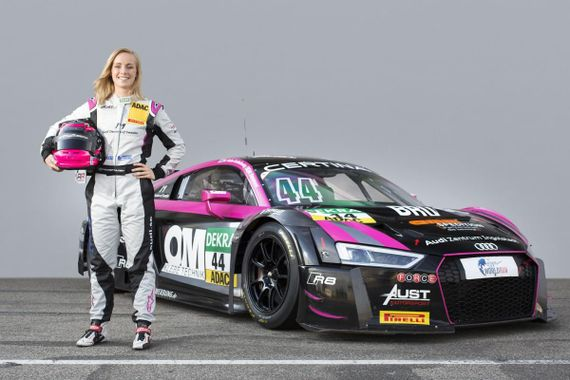
\includegraphics[width=.45\linewidth]{images/race_car_driver}
%\pause
%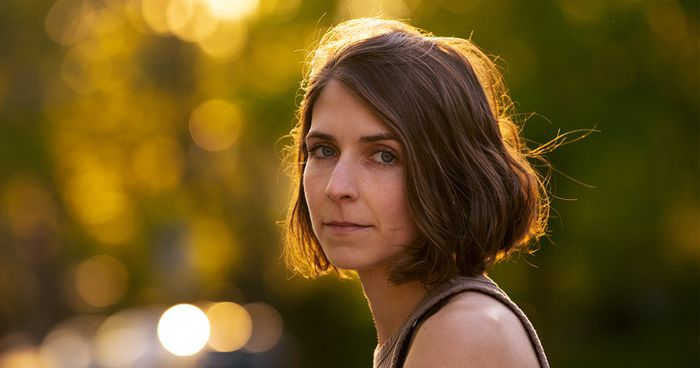
\includegraphics[trim=4.2cm 0 1cm 0,clip, width=.45\linewidth]{images/mathematician}
%
%(you don't need to be a professional driver to drive a car,
%you don't need to be a professional mathematician to use mathematics)
%
%\end{frame}




%\begin{frame}{Bad code hinders reproducibility}
%randomness \onslide<2->{- wherever RNGs are used}
%\begin{itemize}
%\item dataset partitions
%\item initial model state
%\end{itemize}
%
%\pause
%inconsistent conventions \onslide<3->{- causes bugs, difficult to read code}
%\begin{itemize}
%\item variables
%\item naming
%\item organization
%\end{itemize}
%
%\pause
%spaghetti code \onslide<4->{- causes bugs, difficult to read code}
%\begin{itemize}
%\item poor organization
%\item esoteric coding style
%\item overengineered
%\end{itemize}
%
%\end{frame}





\begin{frame}[fragile]{Project Initiation}
Use standard directory structures and consistent naming conventions

\begin{columns}
\begin{column}{.5\textwidth}
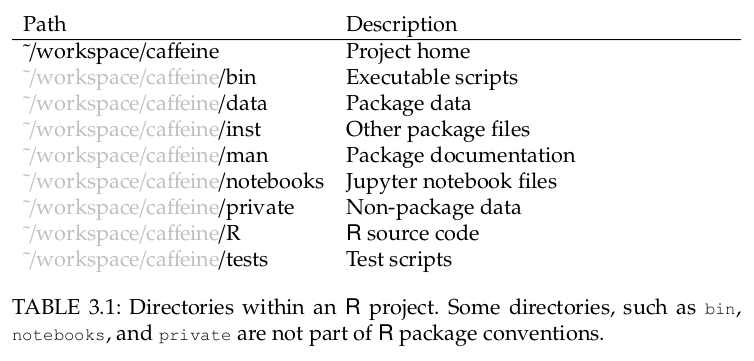
\includegraphics[width=\linewidth]{images/directory_structure}
\end{column}

\begin{column}{.5\textwidth}
\begin{lstlisting}[style=custombash]
#!/bin/bash

project=$1
mkdir -p $project/R $project/tests
cd $project
git init
\end{lstlisting}
\end{column}
\end{columns}
\end{frame}



\begin{frame}[fragile]{Building Code}
Create package, train model, build image

Inaccessible
\begin{lstlisting}[style=custombash]
$ R CMD build --compact-vignettes=gs+qpdf $MY_PACKAGE
\end{lstlisting}

Accessible
\begin{lstlisting}[style=custombash]
$ make build
\end{lstlisting}
\end{frame}



\begin{frame}[fragile]{Testing Code}
Inaccessible
\begin{lstlisting}[style=custombash]
$ R CMD check --as-cran $MY_PACKAGE.tar.gz
$ pytest test
\end{lstlisting}

Accessible
\begin{lstlisting}[style=custombash]
$ make test
\end{lstlisting}

\end{frame}



\begin{frame}[fragile]{Train Model}
Inaccessible
\begin{lstlisting}[style=custombash]
$ Rscript --vanilla -e \
    "library($MY_PACKAGE); \
     withCallingHandlers(train_model($INPUT, $OUTPUT), \
       warning=function(w) stop(w))"
\end{lstlisting}

Accessible
\begin{lstlisting}[style=custombash]
$ make train performance
\end{lstlisting}

\end{frame}


\begin{frame}[fragile]{Run Notebook}
Inaccessible
\begin{lstlisting}[style=custombash]
$ docker run -it -p 8888:8888 $(MOUNT_HOSTDIR) -u jovyan -w /app/$(PACKAGE)/notebooks $(IMAGE) jupyter notebook --allow-root
\end{lstlisting}

Accessible
\begin{lstlisting}[style=custombash]
$ make notebook
\end{lstlisting}

\end{frame}


\begin{frame}[fragile]{Generate Report}
Inaccessible
\begin{lstlisting}[style=custombash]
$ R

> library(rmarkdown)
> rmarkdown::render("reports/myreport.Rmd")
\end{lstlisting}

Accessible
\begin{lstlisting}[style=custombash]
$ make REPORT=reports/myreport.Rmd report
\end{lstlisting}

\end{frame}





\section{Process Automation: Environment}

\begin{frame}{The Computing Environment}

\begin{itemize}
\item Processor
\item Memory
\item Cache
\item Disk
\item Networking
\item Operating system
\item Software dependencies
\item Package dependencies
\end{itemize}

\end{frame}



\begin{frame}{Interlude: Computing History}

\begin{columns}[T]
\begin{column}{.33\linewidth}
1970s

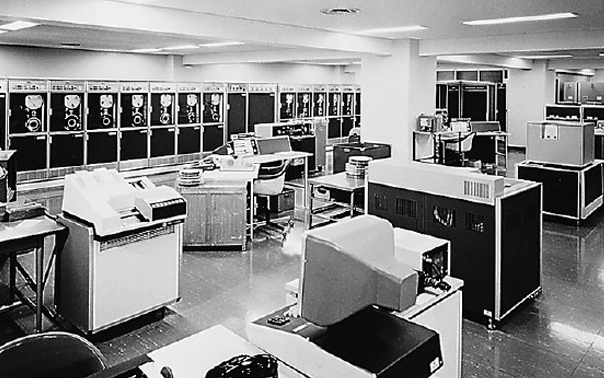
\includegraphics[width=\linewidth]{images/mainframe_1975}

Dumb terminals - mainframes
\end{column}

\begin{column}{.3\linewidth}
late 1970s - 2000s

%https://www.smithsonianmag.com/smithsonian-institution/august-3-1977-the-trs-80-personal-computer-goes-on-sale-186379/
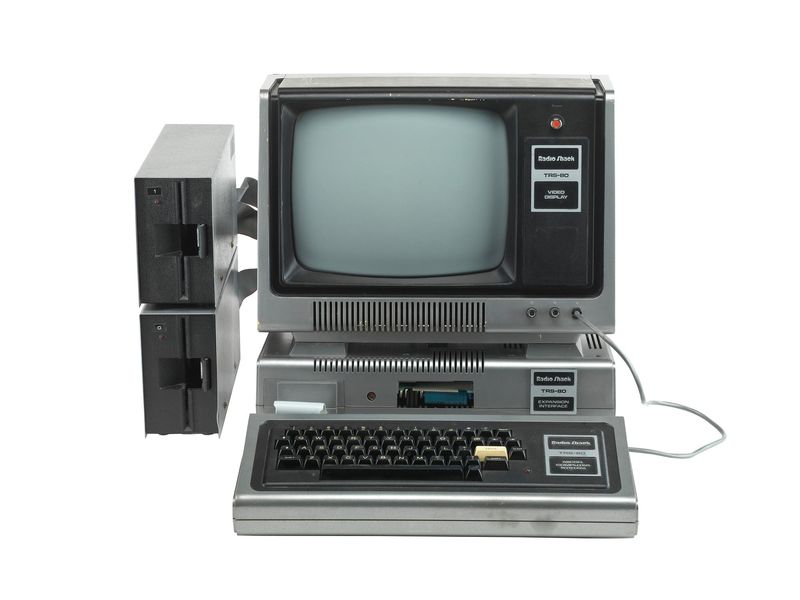
\includegraphics[trim=0 9mm 0 9mm,clip, width=\linewidth]{images/trs-80}

Personal computers
\end{column}

\begin{column}{.33\linewidth}
2000s - present
%https://engineering.fb.com/production-engineering/introducing-data-center-fabric-the-next-generation-facebook-data-center-network/
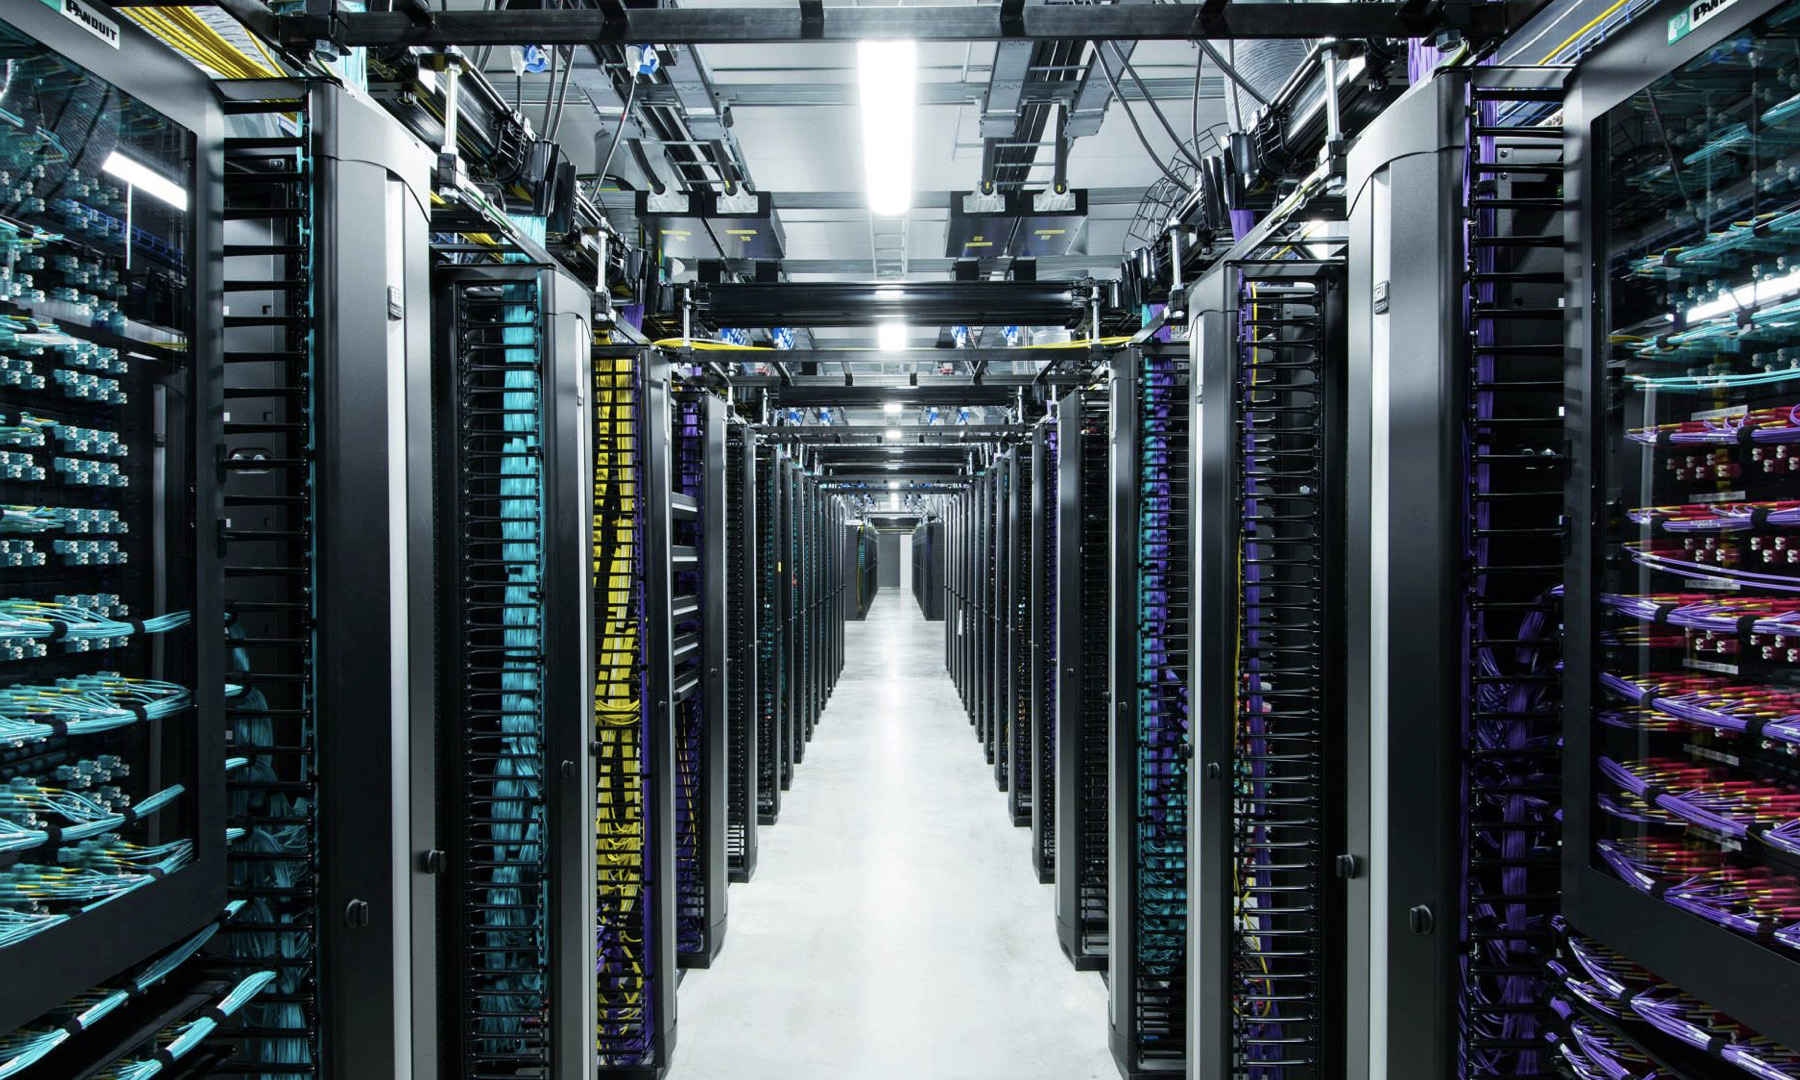
\includegraphics[width=\linewidth]{images/datacenter_fb}

Smart terminals - mainframes
\end{column}
\end{columns}
%\begin{itemize}
%\item Microsoft - Azure
%\item Google - GCP
%\item Amazon - AWS
%\item Others (IBM, et al.)
%\end{itemize}
\end{frame}



\begin{frame}{21st Century Virtual Solution}
\alert{Environment creation and management is virtual and automatable}

\begin{itemize}
\item Cloud IaaS solves hardware issues
\item Containers solve software issues
\end{itemize}

\end{frame}


\begin{frame}{Containers}
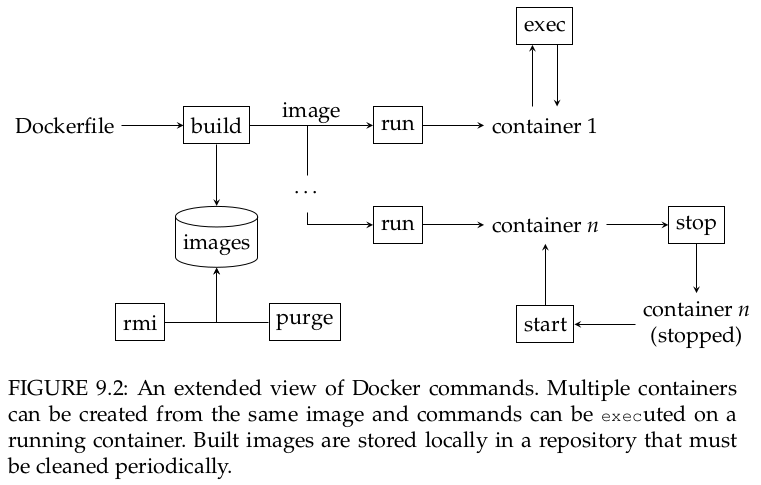
\includegraphics[width=\linewidth]{images/docker_commands}
\end{frame}


\begin{frame}[fragile]{Example: Dockerfile}
Environment creation becomes transparent via automation

\small
\begin{lstlisting}[style=custombash]
FROM jupyter/minimal-notebook:dc9744740e12
MAINTAINER rowe@zatonovo.com

USER root
ENV DEBIAN_FRONTEND noninteractive

RUN \
  apt-get update && \
  apt-get install -qy software-properties-common && \
  add-apt-repository -y ppa:opencpu/opencpu-2.0 && \
  apt-get update && \
  apt-get install -qy opencpu-server x11-apps

# Set opencpu password so that we can login
RUN \
  echo "opencpu:opencpu" | chpasswd
\end{lstlisting}
\end{frame}


\begin{frame}[fragile]{Dependency managers}

System packages (debian)

\small
\begin{lstlisting}[style=custombash]
RUN apt-get install -qy package-1 package-2
\end{lstlisting}

Python packages

\begin{lstlisting}[style=custombash]
RUN pip3 install package-1 package-2
RUN pip3 install -r requirements.txt
\end{lstlisting}

R packages (\href{https://github.com/zatonovo/crant}{crant})

\begin{lstlisting}[style=custombash]
RUN rpackage package-1 package-2
\end{lstlisting}


\end{frame}



\begin{frame}[fragile]{Example: GCP}
% https://cloud.google.com/compute/docs/containers/deploying-containers#gcloud
\begin{lstlisting}[style=custombash]
$ docker build -t [DOCKER_IMAGE] .
$ docker push [DOCKER_IMAGE] .
$ gcloud compute instances \
    create-with-container [INSTANCE_NAME] \
      --container-image [DOCKER_IMAGE]
\end{lstlisting}
\end{frame}


\begin{frame}{Orchestration}
Create collection of connected services

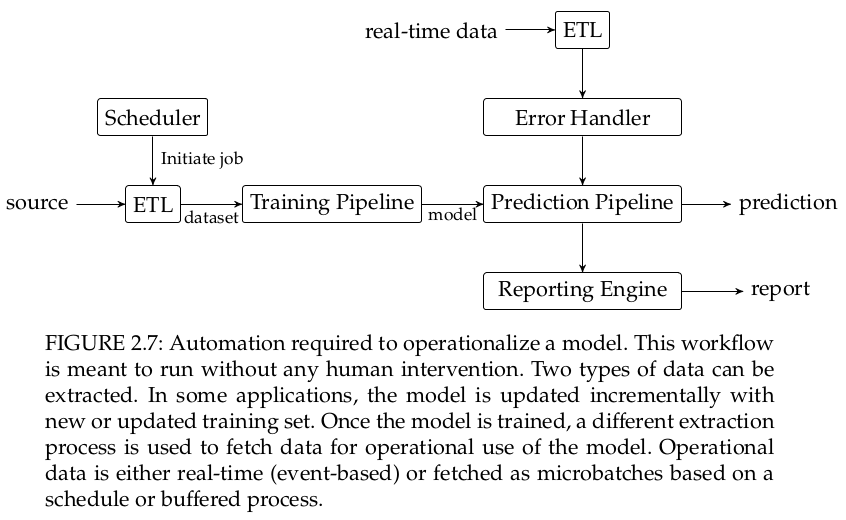
\includegraphics[width=\linewidth]{images/o16n_pipeline}

%Docker Compose
%Kubernetes
\end{frame}




\section{Pearls of Wisdom}

\begin{frame}{Apply Empathy and Consider Others Using Your Code}

Transparent:

\begin{itemize}
\item Self-contained workflows with no hidden (e.g., manual) steps
\item Documentation that explains decisions/rationale for algorithms
\item Consistent, simple code that is easy to read and debug
\item Right tool for job
\end{itemize}

\pause
Accessible:

\begin{itemize}
\item Easy to use end-user interfaces (e.g., make)
\item Dataset easily acquired
\item No human in the loop workflows
\item Minimal dependencies
\item Minimal cost
\end{itemize}

\end{frame}




%\begin{frame}{Reproducibility needs repeatability needs consistency}
%
%Imagine recipe switches between metric and imperial units
%
%Consistency: Conventions are patterns that help our brain. Working memory is shallow.
%%https://www.androidauthority.com/0118-999-881-999-119-725-3-easter-egg-682519/
%
%Repeatability: Re-running jobs due to failures (waiting)
%Debugging is twice as hard as writing code
%
%Reproducibility: Verification is similar to debugging (reading code)
%\end{frame}





\begin{frame}{Assume Everything Will Be Done Again}
Focus on repeatability:

\begin{itemize}
\item Use containers to exactly create your environment
\item Use Linux to simplify scripting/automation
\item Write executable scripts (e.g., bash) to document processes
\item Minimize interactive development
\item Create functions as much as possible
\item Use error handling to avoid frustration
\end{itemize}

\end{frame}


\begin{frame}{Thank You}
Questions: \href{mailto:rowe@zatonovo.com}{rowe@zatonovo.com}

Twitch: @cartesianfaith $\leftarrow$ experiment for live data science/coding help\\
Twitter: @cartesianfaith\\
Personal website: https://cartesianfaith.com

\end{frame}

\appendix

\end{document}
